\documentclass[UTF8,a4paper,11pt]{ctexart}

\usepackage[left=2.5cm,right=2.5cm,top=2.6cm,bottom=2.6cm]{geometry}
\usepackage{amsmath,amssymb,bm}
\usepackage{graphicx}
\usepackage{booktabs,array,multirow}
\usepackage{subcaption}
\usepackage{float}
\usepackage{caption}
\usepackage{xcolor}
\usepackage{hyperref}

\hypersetup{colorlinks=true,linkcolor=blue!45!black,citecolor=blue!45!black,urlcolor=blue!45!black}
\graphicspath{{figures/}}
\captionsetup{font=small,labelfont=bf}
\setlength{\parskip}{0.35em}
\setlength{\parindent}{2em}
\renewcommand{\arraystretch}{1.18}
\newcommand{\RMSE}{\mathrm{RMSE}}
\newcommand{\FWHM}{\mathrm{FWHM}}

\title{\bfseries 光栅光谱仪的波长定标、钠黄双线与量子数亏损\\[0.4em]
\large ——基于 WGD-8A 型光谱仪实验数据}
\author{姓名：\underline{\hspace{3.0cm}}\qquad 学号：\underline{\hspace{3.0cm}}\\[0.5em]
班级：\underline{\hspace{3.0cm}}\qquad 同组人：\underline{\hspace{2.4cm}}}
\date{\today}

\begin{document}
\maketitle

\begin{abstract}
本实验利用 WGD-8A 型组合式多功能光栅光谱仪采集的汞灯、钠灯和绿激光数据，研究波长定标、钠黄双线、狭缝宽度对表观分辨能力的影响，以及钠原子里德伯能级的量子数亏损。选取 6 条可见汞线建立线性定标关系，得到 $\lambda_{\mathrm{cal}}=(0.989277\lambda_{\mathrm{read}}+6.133789)\ \mathrm{nm}$，定标残差均方根为 $0.0419\ \mathrm{nm}$。对 $0.5$、$1.0$、$1.5\ \mathrm{mm}$ 狭缝下的钠黄双线进行双高斯拟合，测得两条谱线平均波长分别为 $(589.030\pm0.042)\ \mathrm{nm}$ 和 $(589.628\pm0.042)\ \mathrm{nm}$，平均间距为 $(0.59755\pm0.00571)\ \mathrm{nm}$，与标准间距的相对偏差为 $0.024\%$。狭缝由 $0.5\ \mathrm{mm}$ 增至 $2.5\ \mathrm{mm}$ 时，谱线或合并谱带的半高宽总体由 $0.367\ \mathrm{nm}$ 增至约 $1.024\ \mathrm{nm}$，$2.0\ \mathrm{mm}$ 及以上双线不再可分辨。利用钠原子全谱中的 $3p\to ns$（$n=5,6,7,8$）和 $3p\to nd$（$n=4,5,6$）系列，计算有效量子数与量子数亏损，得到 $\bar\delta_s=1.33905$，Ritz 外推参数 $\delta_0=1.32056\pm0.00861$；饱和 $d$ 系列按多重态平均估算得 $\bar\delta_d=0.00852$。绿激光文件的有效扫描段在预期的 $532\ \mathrm{nm}$ 位置未出现可识别主峰，故该文件不用于定标。
\end{abstract}

\noindent\textbf{关键词：}光栅光谱仪；波长定标；钠黄双线；里德伯能级；量子数亏损；狭缝宽度

\section{实验目的}
\begin{enumerate}
  \item 理解光栅色散与光谱仪器分辨本领的基本原理，掌握波长扫描数据的处理方法。
  \item 利用汞灯特征谱线建立仪器读数波长与标准波长之间的定标关系。
  \item 测量钠黄双线 $D_2$、$D_1$ 的波长及其间距，并与标准值比较。
  \item 指认钠原子 $3p\to ns$ 和 $3p\to nd$ 里德伯系列，计算各能级的量子数亏损并进行 Ritz 拟合。
  \item 研究入射狭缝宽度对谱线半高宽和双线可分辨程度的影响。
  \item 检查绿激光扫描数据，分析饱和、杂散光及文件分段对实验结果的影响。
\end{enumerate}

\section{实验原理}
\subsection{光栅色散与分辨本领}
光栅方程为
\begin{equation}
  d(\sin i+\sin\theta)=m\lambda,
  \label{eq:grating}
\end{equation}
其中 $d$ 为光栅常数，$i$ 和 $\theta$ 分别为入射角和衍射角，$m$ 为衍射级次，$\lambda$ 为波长。固定入射条件时，不同波长的光在空间上分开，转动光栅或探测机构即可得到波长扫描谱。

角色散和理论分辨本领分别为
\begin{equation}
  \frac{\mathrm{d}\theta}{\mathrm{d}\lambda}=\frac{m}{d\cos\theta},
  \qquad R=\frac{\lambda}{\Delta\lambda}=mN,
\end{equation}
其中 $N$ 为被照亮的刻线数。实际测得的线宽还受狭缝宽度、像差、探测器响应和采样间隔影响。因此，本报告由实测半高宽计算的 $R_{\mathrm{eff}}=\lambda/\FWHM$ 仅表示\textbf{表观分辨指标}，不等同于理想光栅的 $mN$。

\subsection{波长定标}
以汞灯标准波长 $\lambda_{\mathrm{ref}}$ 对仪器读数波长 $\lambda_{\mathrm{read}}$ 作线性最小二乘拟合：
\begin{equation}
  \lambda_{\mathrm{cal}}=a\lambda_{\mathrm{read}}+b.
  \label{eq:calibration}
\end{equation}
拟合残差均方根定义为
\begin{equation}
  \RMSE=\sqrt{\frac{1}{n}\sum_{j=1}^{n}\left[\lambda_{\mathrm{ref},j}-(a\lambda_{\mathrm{read},j}+b)\right]^2}.
  \label{eq:rmse}
\end{equation}
本报告用该 $\RMSE$ 估计定标后单条谱线波长的典型不确定度。定标直线的高 $R^2$ 只说明线性相关程度，波长偏差仍应结合残差判断。

\subsection{谱线拟合与半高宽}
对可分辨的钠黄双线采用无常数背景的双高斯模型：
\begin{equation}
  I(\lambda)=A_1\exp\!\left[-\frac{(\lambda-c_1)^2}{2\sigma_1^2}\right]
  +A_2\exp\!\left[-\frac{(\lambda-c_2)^2}{2\sigma_2^2}\right].
  \label{eq:double_gaussian}
\end{equation}
$c_1,c_2$ 为读数波长下的峰位。单条高斯谱线的半高宽为
\begin{equation}
  \FWHM=2\sqrt{2\ln2}\,\sigma.
\end{equation}
$0.5$--$1.5\ \mathrm{mm}$ 数据中分别报告两条谱线的宽度并取平均；$2.0$ 和 $2.5\ \mathrm{mm}$ 数据已无两个独立峰，故仅以单高斯近似整个谱带，其宽度用于说明展宽趋势，不用于反推双线间距。

\subsection{里德伯能级与量子数亏损}
碱金属原子的价电子能级偏离氢原子能级，可用有效量子数 $n^*=n-\delta_l$ 表示。以波数为单位，$nl$ 能级及其结合能（项能）写为
\begin{equation}
  E_{nl}=E_\infty-\frac{R_{\mathrm{Na}}}{(n-\delta_l)^2},
  \qquad T_{nl}=E_\infty-E_{nl}=\frac{R_{\mathrm{Na}}}{(n-\delta_l)^2},
  \label{eq:rydberg}
\end{equation}
其中 $E_\infty$ 为电离限，$R_{\mathrm{Na}}$ 为考虑有限原子核质量后的里德伯常量，$\delta_l$ 为角量子数 $l$ 对应系列的量子数亏损。

对于发射跃迁 $nl\to3p$，测得波长 $\lambda$（单位：$\mathrm{nm}$）对应波数 $\tilde\nu=10^7/\lambda$（单位：$\mathrm{cm^{-1}}$）。于是
\begin{equation}
  T_{nl}=E_\infty-E_{3p}-\tilde\nu,
  \qquad n^*=\sqrt{\frac{R_{\mathrm{Na}}}{T_{nl}}},
  \qquad \delta_l=n-n^*.
  \label{eq:quantum_defect}
\end{equation}
本计算取 $E_\infty=41449.451\ \mathrm{cm^{-1}}$、$R_{\mathrm{Na}}=109734.716\ \mathrm{cm^{-1}}$；$3p_{1/2}$ 和 $3p_{3/2}$ 能级分别为 $16956.172$ 和 $16973.368\ \mathrm{cm^{-1}}$\cite{na_levels}。$s$ 系列统一使用短波成分，即下能级 $3p_{3/2}$；饱和的 $d$ 系列采用两个下能级的算术平均 $\bar E_{3p}=16964.770\ \mathrm{cm^{-1}}$。

量子数亏损的高阶修正可用 Ritz 展开近似：
\begin{equation}
  \delta_l(n)=\delta_0+\frac{A_l}{(n-\delta_0)^2},
  \label{eq:ritz}
\end{equation}
其中 $\delta_0$ 表示 $n\to\infty$ 时的极限值。由式~\eqref{eq:quantum_defect} 可得波长误差的一阶传播关系
\begin{equation}
  u(\delta_l)\approx\frac{n^*\,10^7}{2T_{nl}\lambda^2}\,u(\lambda),
  \label{eq:delta_uncertainty}
\end{equation}
因此，高 $n$ 能级的 $T_{nl}$ 较小，其量子数亏损对波长误差更敏感。

\section{实验仪器与数据}
实验数据文件头显示仪器为 WGD-8A 型组合式多功能光栅光谱仪，采集模式为能量模式，每次扫描采集 5 次。光源包括汞灯、钠灯和绿激光器。原始数据均为两列文本：第一列为读数波长（$\mathrm{nm}$），第二列为相对强度（任意单位）。表~\ref{tab:data} 列出本报告实际使用的扫描区间。

\begin{table}[H]
  \centering
  \caption{原始数据及扫描参数}
  \label{tab:data}
  \small
  \begin{tabular}{lllll}
    \toprule
    数据目录 & 文件 & 使用区间/$\mathrm{nm}$ & 间隔/$\mathrm{nm}$ & 狭缝/$\mathrm{mm}$ \\
    \midrule
    Hg-all & 0.35mm.txt & 250--660 & 0.05 & 0.35 \\
    Na-all & 0.35mm.txt & 450--650 & 0.01 & 0.35 \\
    Na-589 & 0.5mm.txt & 588--590 & 0.01 & 0.5 \\
    Na-589 & 1.0.txt & 588--590 & 0.01 & 1.0 \\
    Na-589 & 1.5mm.txt & 588--590 & 0.01 & 1.5 \\
    Na-589 & 2.0mm.txt & 588--590 & 0.01 & 2.0 \\
    Na-589 & 2.5mm.txt & 588--590 & 0.01 & 2.5 \\
    LASER & green.txt & 480--570 & 0.50 & 未记录 \\
    \bottomrule
  \end{tabular}
\end{table}

钠灯变狭缝文件还包含 $500.93$--$588\ \mathrm{nm}$ 的其他分段，这些分段在各狭缝文件中基本重复；本实验仅使用文件头指定的第三段 $588$--$590\ \mathrm{nm}$ 研究钠黄双线。绿激光文件包含 4 个分段，本报告只将 $480$--$570\ \mathrm{nm}$ 的第三段视为该次绿激光检查的有效扫描段。

\section{数据处理与结果}
\subsection{汞灯全谱与线性定标}
图~\ref{fig:hg_spectrum} 给出汞灯全谱。可见区多条强线达到 $996.3$ 的强度上限，出现平顶。为避免饱和峰形对峰位的影响，对具有平顶的谱线取最高强度平台对应读数波长的中点；对未饱和单峰取局部极大值。定标只使用峰位，不使用峰高或峰面积。

\begin{figure}[H]
  \centering
  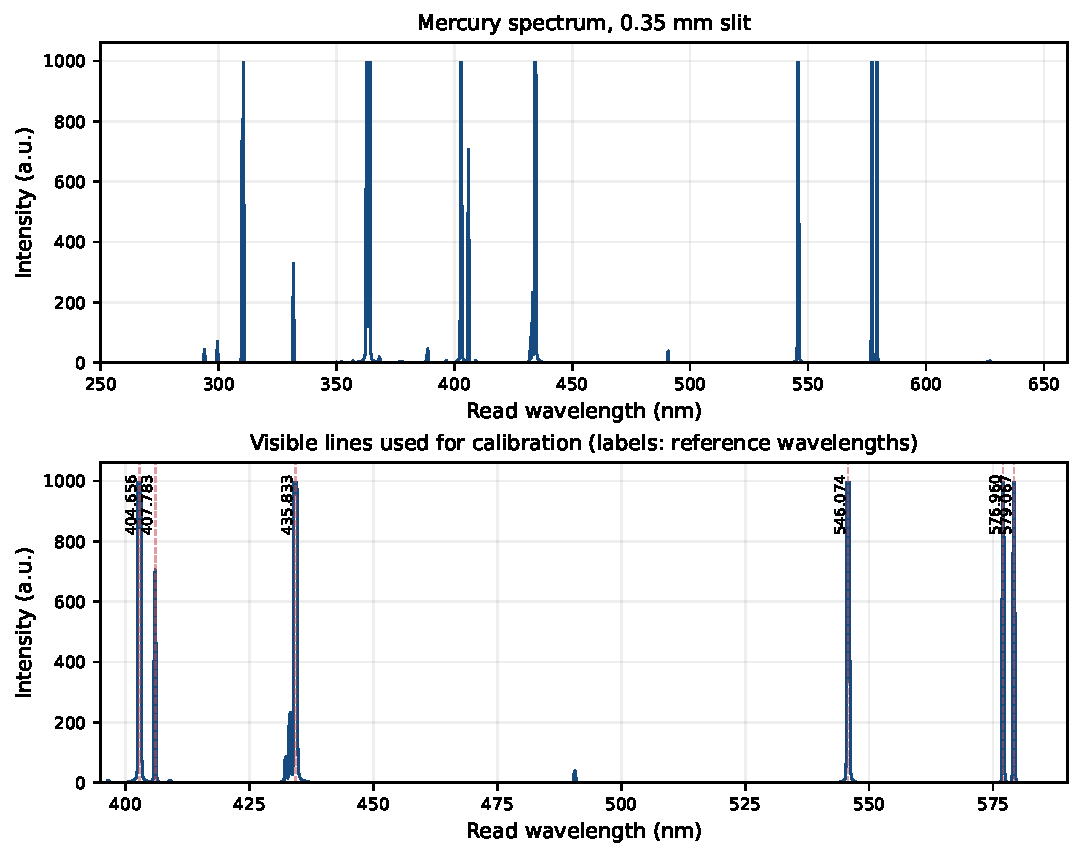
\includegraphics[width=0.70\textwidth]{hg_spectrum.pdf}
  \caption{汞灯全谱及用于定标的可见谱线。下图中标注为标准波长，竖线位置为原始读数波长。}
  \label{fig:hg_spectrum}
\end{figure}

选取 $404.656$、$407.783$、$435.833$、$546.074$、$576.960$ 和 $579.067\ \mathrm{nm}$ 六条汞线，标准值取自 NIST 原子光谱数据库\cite{nist}，结果见表~\ref{tab:hg_calibration}。线性拟合得到
\begin{equation}
  \boxed{\lambda_{\mathrm{cal}}=0.9892773768\,\lambda_{\mathrm{read}}+6.1337889352}
  \label{eq:calibration_result}
\end{equation}
式中波长均以 $\mathrm{nm}$ 为单位。拟合优度 $R^2=0.99999970$，由式~\eqref{eq:rmse} 得 $\RMSE=0.04186\ \mathrm{nm}$。图~\ref{fig:hg_calibration} 显示残差在 $\pm0.06\ \mathrm{nm}$ 内，未见需要高阶经验修正的明显趋势。

\begin{table}[H]
  \centering
  \caption{汞灯特征谱线的定标数据}
  \label{tab:hg_calibration}
  \small
  \begin{tabular}{cccc}
    \toprule
    标准波长/$\mathrm{nm}$ & 读数波长/$\mathrm{nm}$ & 峰值强度/任意单位 & 拟合残差/$\mathrm{nm}$ \\
    \midrule
    404.656 & 402.85 & 996.3 & $-0.008$ \\
    407.783 & 406.05 & 705.5 & $-0.047$ \\
    435.833 & 434.30 & 996.3 & $+0.056$ \\
    546.074 & 545.75 & 996.3 & $+0.042$ \\
    576.960 & 577.00 & 996.3 & $+0.013$ \\
    579.067 & 579.20 & 996.3 & $-0.056$ \\
    \bottomrule
  \end{tabular}
\end{table}

\begin{figure}[H]
  \centering
  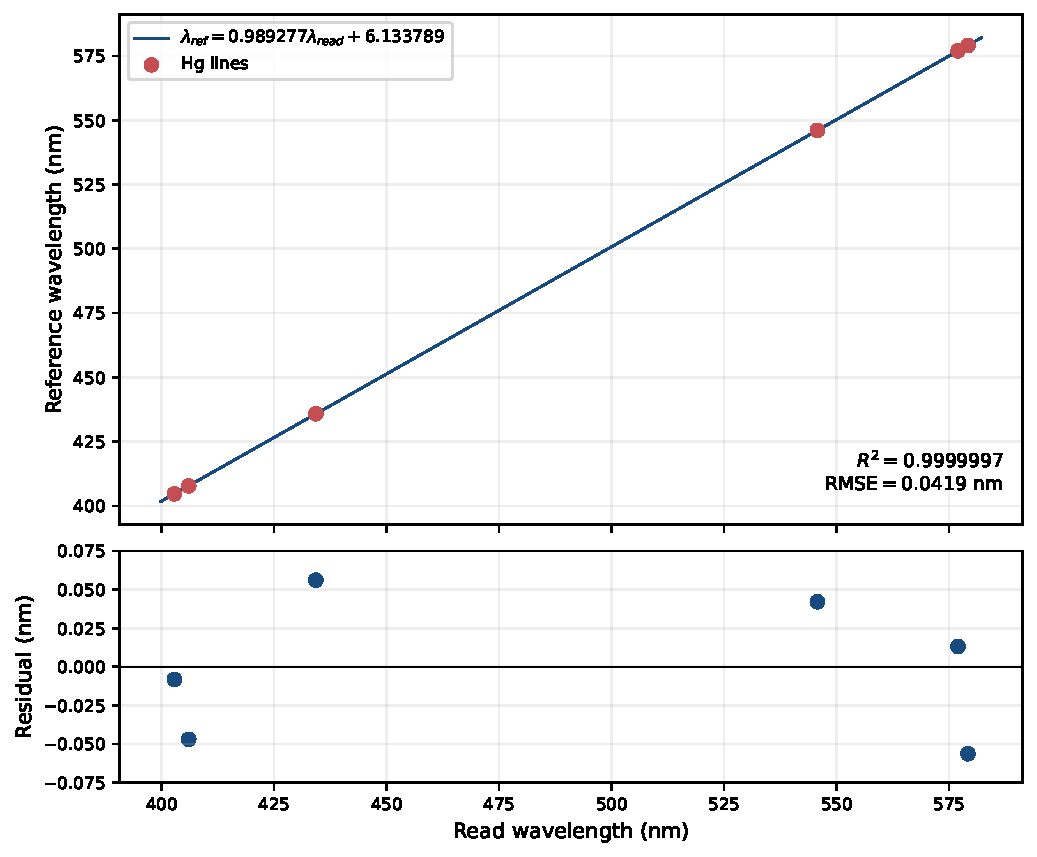
\includegraphics[width=0.84\textwidth]{hg_calibration.pdf}
  \caption{汞灯线性定标及残差。}
  \label{fig:hg_calibration}
\end{figure}

\subsection{钠灯全谱的饱和检查}
图~\ref{fig:na_overview} 显示 $0.35\ \mathrm{mm}$ 狭缝下的钠灯全谱。$588.15$--$590.85\ \mathrm{nm}$ 附近强度持续处于 $996.3$ 上限，双线峰形完全饱和；此外，若干其他波段也出现饱和平台。因此，该全谱文件用于展示光谱分布和检查饱和，不用于提取钠黄双线峰位、线宽或相对强度。

\begin{figure}[H]
  \centering
  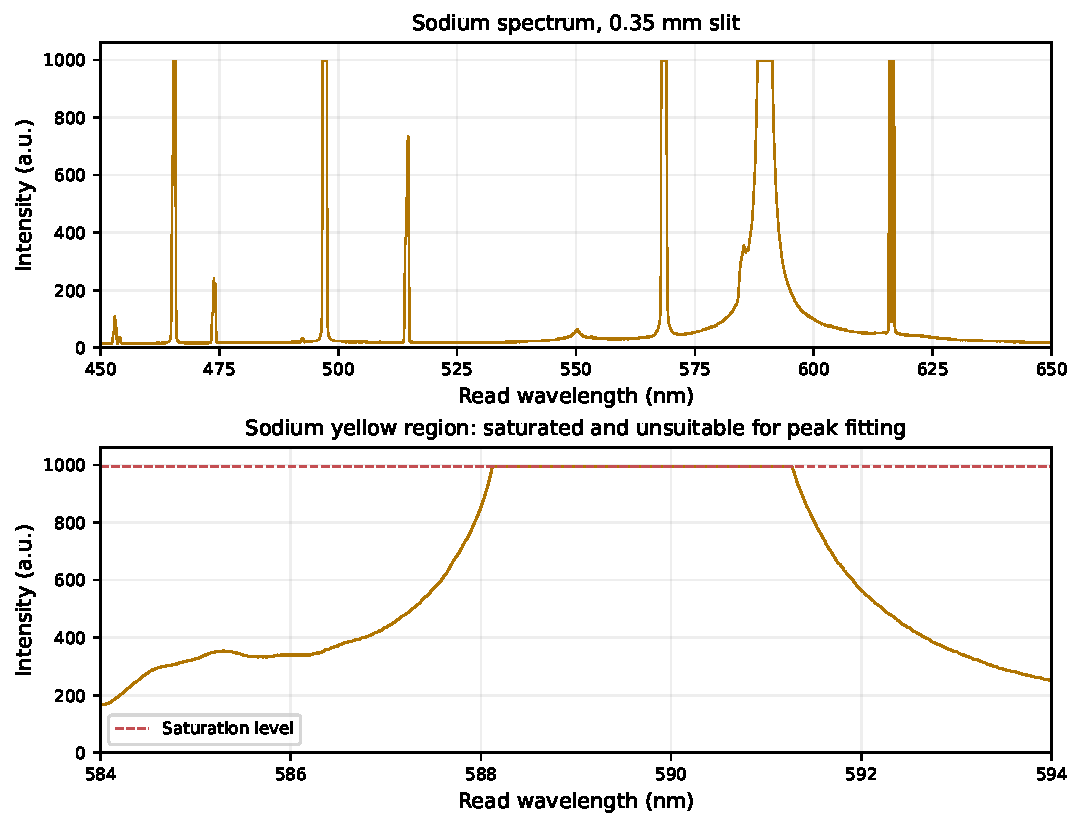
\includegraphics[width=0.75\textwidth]{na_overview.pdf}
  \caption{钠灯全谱及黄光区饱和情况。}
  \label{fig:na_overview}
\end{figure}

\subsection{钠原子全谱与量子数亏损}
除饱和的钠黄区外，全谱中还可指认 $3p\to ns$ 锐线系和 $3p\to nd$ 漫线系。本文件的扫描范围为 $450$--$650\ \mathrm{nm}$，故可使用 $5s$ 至 $8s$、$4d$ 至 $6d$；$7d$ 对应谱线位于扫描下限之外，未纳入计算。谱线指认与参考波长均依据 NIST 原子光谱数据\cite{nist}，图~\ref{fig:na_quantum_defect} 标出了所用系列。

对于 $s$ 系列，统一使用下能级为 $3p_{3/2}$ 的短波成分。$5s$ 和 $6s$ 分别取对应峰值平台的中心，$7s$ 和 $8s$ 的短波峰与长波肩部采用含常数背景的双高斯模型拟合。对于饱和的 $d$ 系列，平台覆盖了双重态，无法可靠分离两个精细结构成分，因此取整个饱和平台的中心，并以 $3p$ 两个下能级的平均值作多重态估算。参考量子数亏损 $\delta_{\mathrm{ref}}$ 是用参考波长代入同一公式得到的比较值，而非额外拟合参数。

\begin{table}[H]
  \centering
  \caption{钠原子里德伯系列的项能、有效量子数和量子数亏损}
  \label{tab:quantum_defect}
  \small
  \resizebox{\textwidth}{!}{%
  \begin{tabular}{ccccccc}
    \toprule
    系列与跃迁 & 测量波长/$\mathrm{nm}$ & 波数/$\mathrm{cm^{-1}}$ & 项能 $T_{nl}$/$\mathrm{cm^{-1}}$ & $n^*$ & $\delta_l$ & $\delta_{\mathrm{ref}}$ \\
    \midrule
    $3p_{3/2}\leftarrow5s$ & 615.529 & 16246.197 & 8229.886 & 3.65153 & 1.34847 & 1.34785 \\
    $3p_{3/2}\leftarrow6s$ & 515.315 & 19405.612 & 5070.471 & 4.65209 & 1.34791 & 1.34835 \\
    $3p_{3/2}\leftarrow7s$ & 474.897 & 21057.189 & 3418.894 & 5.66538 & 1.33462 & 1.33082 \\
    $3p_{3/2}\leftarrow8s$ & 454.276 & 22013.063 & 2463.020 & 6.67480 & 1.32520 & 1.31779 \\
    \midrule
    $3p(\mathrm{mean})\leftarrow4d$ & 568.493 & 17590.352 & 6894.329 & 3.98957 & 0.01043 & 0.01087 \\
    $3p(\mathrm{mean})\leftarrow5d$ & 497.938 & 20082.814 & 4401.867 & 4.99291 & 0.00709 & 0.01011 \\
    $3p(\mathrm{mean})\leftarrow6d$ & 466.672 & 21428.323 & 3056.358 & 5.99197 & 0.00803 & 0.00804 \\
    \bottomrule
  \end{tabular}}
\end{table}

表~\ref{tab:quantum_defect} 中，$s$ 系列的四个量子数亏损为 $1.32520$--$1.34847$，平均值及离散性为
\begin{equation}
  \bar\delta_s=1.33905,\qquad s(\delta_s)=0.01123.
\end{equation}
这里的标准差主要包含量子数亏损随 $n$ 的实际变化，不能全部视为随机测量误差。按式~\eqref{eq:ritz} 拟合得到
\begin{equation}
  \boxed{\delta_s(n)=1.32056+\frac{0.42750}{(n-1.32056)^2}},
\end{equation}
其中 $\delta_0=1.32056\pm0.00861$、$A_s=0.42750\pm0.18296$，拟合均方根残差为 $0.00499$。该结果说明 $s$ 电子显著穿透原子实，能级明显偏离氢原子；且高阶修正不可完全忽略。

$d$ 系列多重态估算的平均值为
\begin{equation}
  \boxed{\bar\delta_d=0.00852,\qquad s(\delta_d)=0.00172}.
\end{equation}
其数值接近零，符合 $d$ 电子受原子实穿透和极化影响较小的物理图像。$5d$ 的测量值与参考计算值相差 $-0.00302$，大于仅由定标 $\RMSE$ 传播的约 $0.00096$，主要反映饱和平台中心和多重态平均近似带来的系统误差。因此，$d$ 系列结果应作为估算，而不宜报告过高的有效数字精度。

\begin{figure}[H]
  \centering
  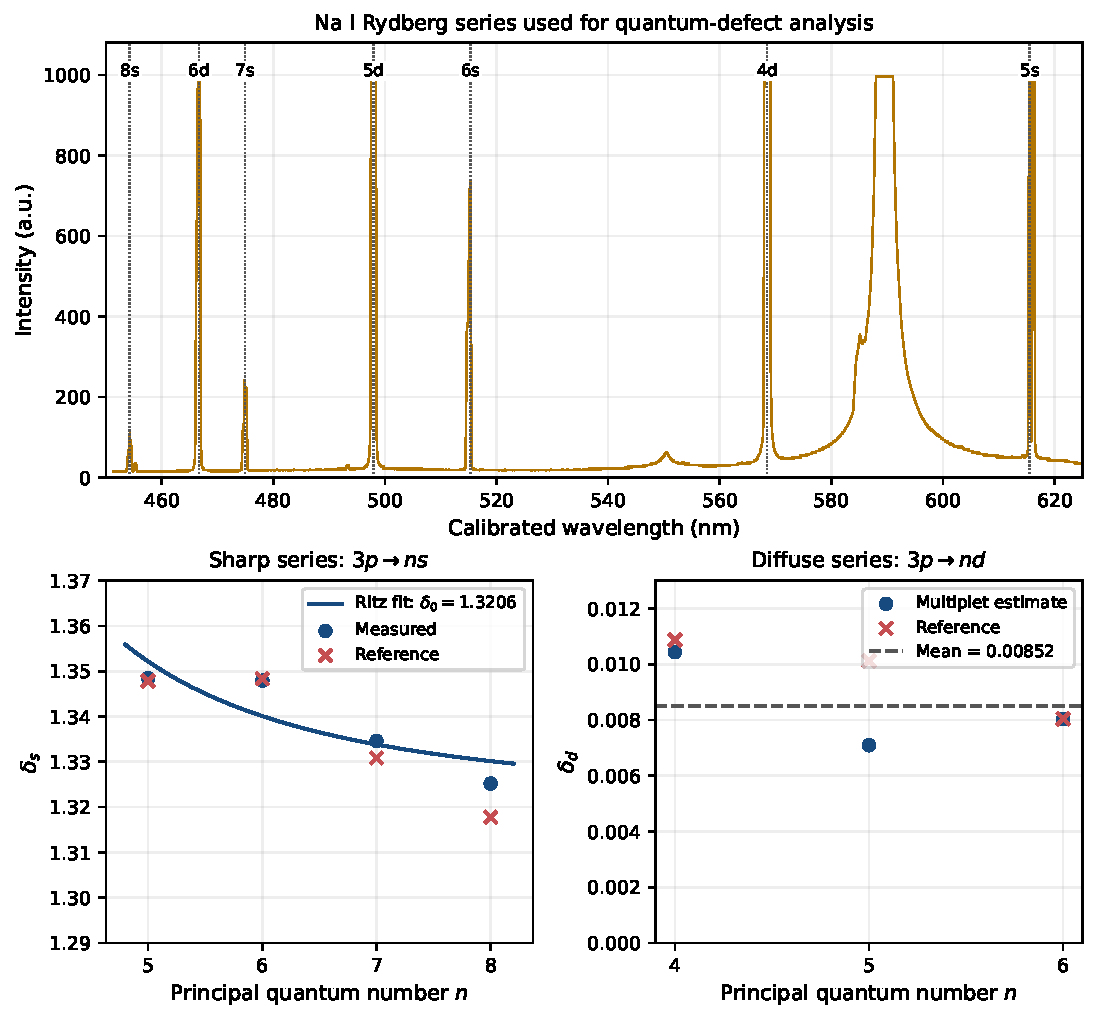
\includegraphics[width=0.92\textwidth]{na_quantum_defect.pdf}
  \caption{钠原子里德伯系列指认及量子数亏损。上图为定标后的全谱；下图圆点为测量值，叉号为参考波长计算值，实线为 $s$ 系列 Ritz 拟合。}
  \label{fig:na_quantum_defect}
\end{figure}

\subsection{钠黄双线波长与间距}
对变狭缝扫描的有效区间 $588$--$590\ \mathrm{nm}$ 进行拟合，再由式~\eqref{eq:calibration_result} 修正峰位。拟合结果见图~\ref{fig:na_slits} 和表~\ref{tab:na_slits}。短波长线记为 $D_2$，长波长线记为 $D_1$。

\begin{figure}[H]
  \centering
  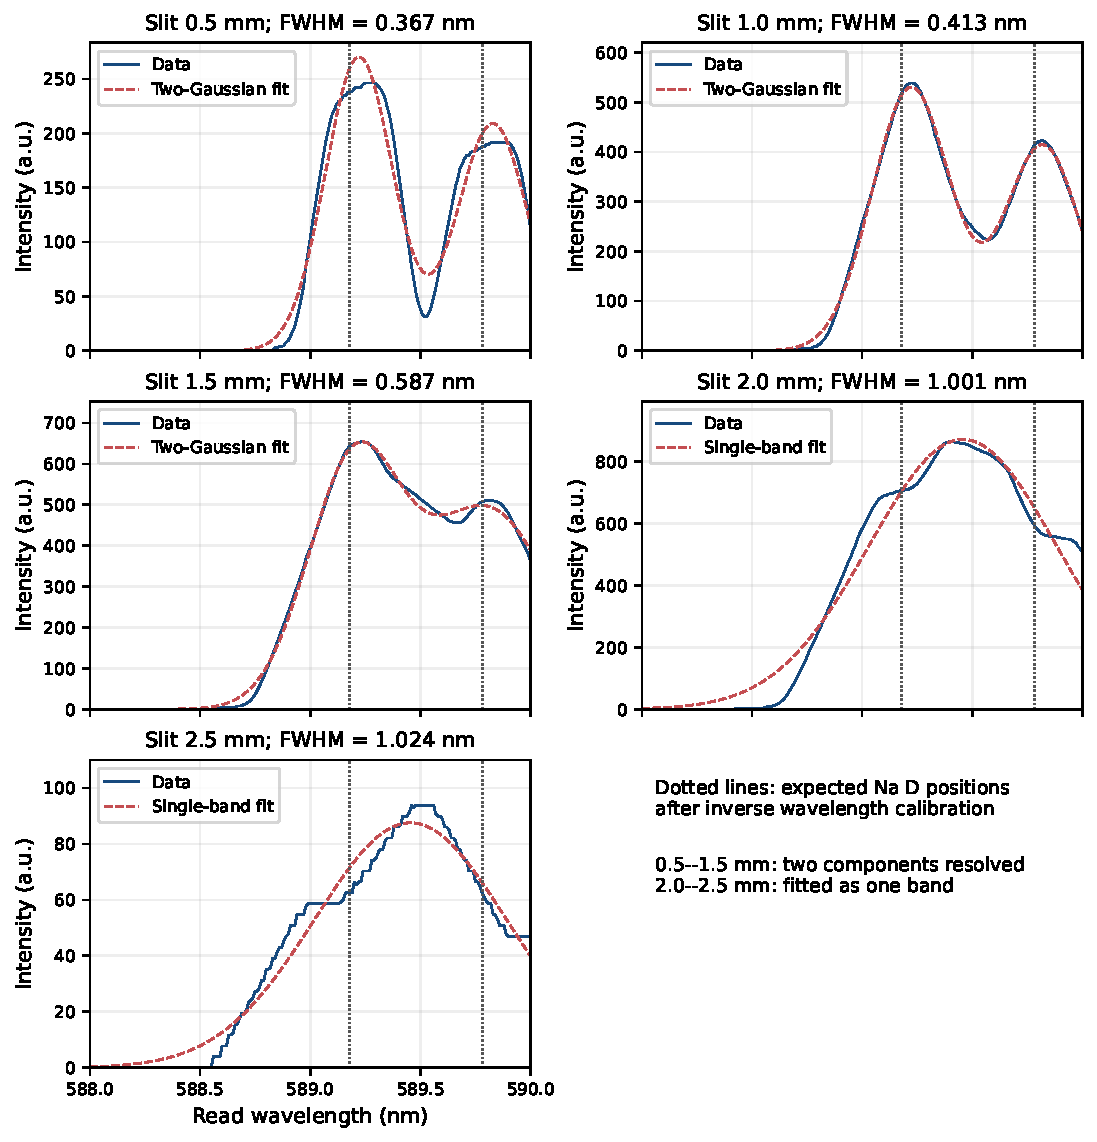
\includegraphics[width=0.94\textwidth]{na_slits.pdf}
  \caption{不同狭缝宽度下的钠黄双线及拟合。点线为定标后标准双线位置对应的原始读数位置。}
  \label{fig:na_slits}
\end{figure}

\begin{table}[H]
  \centering
  \caption{不同狭缝宽度下的拟合结果}
  \label{tab:na_slits}
  \small
  \resizebox{\textwidth}{!}{%
  \begin{tabular}{cccccccc}
    \toprule
    狭缝/$\mathrm{mm}$ & $\lambda_{D_2}$/$\mathrm{nm}$ & $\lambda_{D_1}$/$\mathrm{nm}$ & $\Delta\lambda$/$\mathrm{nm}$ & $\FWHM$/$\mathrm{nm}$ & $R_{\mathrm{eff}}$ & 峰形判断 & 拟合残差/任意单位 \\
    \midrule
    0.5 & 589.037 & 589.638 & 0.6007 & 0.3665 & 1608 & 双峰可分辨 & 15.1 \\
    1.0 & 589.038 & 589.629 & 0.5910 & 0.4126 & 1428 & 双峰可分辨 & 7.6 \\
    1.5 & 589.016 & 589.617 & 0.6010 & 0.5872 & 1004 & 双峰可分辨 & 12.3 \\
    2.0 & --- & --- & --- & 1.0011 & 589 & 合并谱带 & 53.0 \\
    2.5 & --- & --- & --- & 1.0236 & 576 & 合并谱带 & 5.4 \\
    \bottomrule
  \end{tabular}}
\end{table}

注：前三行的 $\FWHM$ 为两条高斯分量半高宽的平均值，后两行为整个谱带的单高斯近似宽度。$R_{\mathrm{eff}}$ 统一以 $589.3\ \mathrm{nm}$ 除以相应宽度估算，只用于比较本组数据。

取三个可分辨狭缝条件的算术平均，得到
\begin{align}
  \lambda_{D_2}&=589.03045\ \mathrm{nm},\\
  \lambda_{D_1}&=589.62799\ \mathrm{nm},\\
  \overline{\Delta\lambda}&=0.5975458\ \mathrm{nm}.
\end{align}
三次间距的样本标准差为 $0.0057059\ \mathrm{nm}$。以定标 $\RMSE$ 作为单线波长的典型不确定度，最终结果写为
\begin{equation}
  \boxed{\lambda_{D_2}=(589.030\pm0.042)\ \mathrm{nm},\qquad
  \lambda_{D_1}=(589.628\pm0.042)\ \mathrm{nm}}
\end{equation}
和
\begin{equation}
  \boxed{\overline{\Delta\lambda}=(0.59755\pm0.00571)\ \mathrm{nm}}.
\end{equation}
这里的间距不确定度为不同狭缝结果之间的离散性，不包含所有系统误差。NIST 给出的空气中波长为 $588.9950\ \mathrm{nm}$ 和 $589.5924\ \mathrm{nm}$\cite{nist}，对应标准间距 $0.59740\ \mathrm{nm}$。本实验两条谱线分别偏高 $0.03545$ 和 $0.03560\ \mathrm{nm}$，均在定标残差量级内；间距的相对偏差为
\begin{equation}
  \frac{0.5975458-0.59740}{0.59740}\times100\%=0.0244\%.
\end{equation}
两条谱线具有相近的同向偏差，而间距仍高度一致，说明共同的波长零点或定标偏移是主要表观误差，峰间色散在本次测量精度内较稳定。

\subsection{狭缝宽度对表观分辨能力的影响}
图~\ref{fig:na_width} 显示谱线或谱带半高宽随狭缝增宽而增大。$0.5$--$1.5\ \mathrm{mm}$ 时可观察到两个局部极大值及中间谷，双线可分辨；$2.0\ \mathrm{mm}$ 时仅余肩部和单峰，$2.5\ \mathrm{mm}$ 时为单一宽峰，故这两种条件按不可分辨处理。

狭缝变宽会增加通光量，但同时使不同波长的像在探测器上重叠，导致线宽增大、$R_{\mathrm{eff}}$ 减小。就本组数据而言，$1.0\ \mathrm{mm}$ 在信号强度和双线分辨之间表现较均衡。不同文件的显示量程设置并不相同，因此不对峰高的绝对强弱作定量比较。

\begin{figure}[H]
  \centering
  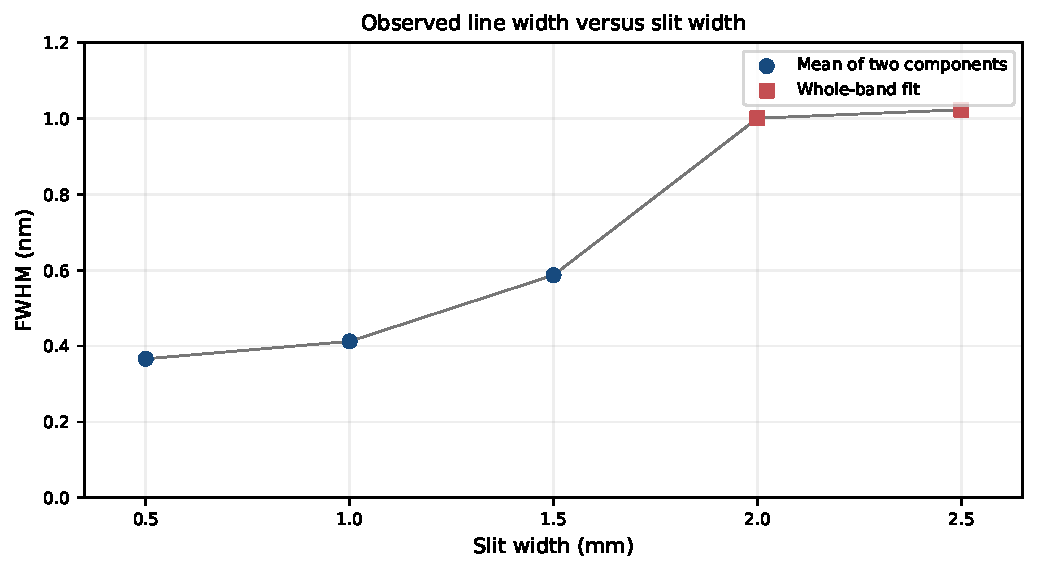
\includegraphics[width=0.82\textwidth]{na_width.pdf}
  \caption{谱线或合并谱带半高宽随狭缝宽度的变化。}
  \label{fig:na_width}
\end{figure}

\subsection{绿激光扫描文件检查}
若绿激光标准波长取 $532\ \mathrm{nm}$，由汞灯定标式反算，其预期读数位置为
\begin{equation}
  \lambda_{\mathrm{read}}=\frac{532-b}{a}=531.566\ \mathrm{nm}.
\end{equation}
但图~\ref{fig:laser_check} 中该位置强度为 0；有效扫描段的最大点仅为 $512.5\ \mathrm{nm}$、$11.7$ 任意单位，无法据此确认 $532\ \mathrm{nm}$ 激光谱线。文件的其他分段还保留了与汞灯扫描相似的峰，说明必须按文件头分段解释数据。

因此，本实验不将 green.txt 用于波长定标，也不报告所谓“测得绿激光波长为 $512.5\ \mathrm{nm}$”。现有证据只能说明该文件中未记录到符合预期的绿激光主峰。可能原因包括激光未正确入射、光路偏折、信号量程或增益不合适、扫描段设置错误，以及文件保存或导出异常。建议检查光源和光路后，以较小扫描间隔重新采集 $500$--$560\ \mathrm{nm}$ 光谱。

\begin{figure}[H]
  \centering
  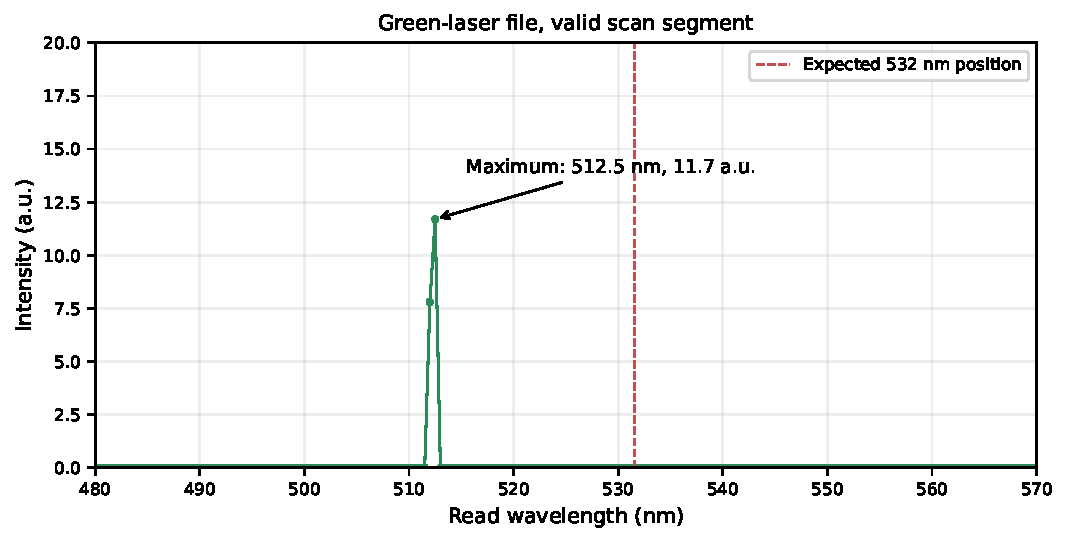
\includegraphics[width=0.88\textwidth]{laser_check.pdf}
  \caption{绿激光文件有效扫描段检查。虚线为 $532\ \mathrm{nm}$ 经定标反算的预期位置。}
  \label{fig:laser_check}
\end{figure}

\section{误差与数据质量讨论}
\begin{enumerate}
  \item \textbf{探测器饱和：}汞灯强线和钠灯全谱在 $996.3$ 处出现平顶，丢失真实峰形和强度信息。饱和谱线只能谨慎提取平台中心，钠灯全谱不能用于钠黄双线拟合。后续实验应降低增益、负高压或入射光强。
  \item \textbf{定标与峰位误差：}线性定标的 $\RMSE=0.0419\ \mathrm{nm}$，与钠双线的共同偏差约 $0.036\ \mathrm{nm}$ 同量级。采样间隔、标准波长口径及饱和平台中心估计也会影响结果。
  \item \textbf{量子数亏损的系统误差：}由式~\eqref{eq:delta_uncertainty} 可知，高 $n$ 能级对波长偏差更敏感。$d$ 系列还存在饱和平台中心不等于多重态强度重心的问题，因此其平均值主要作定性及半定量比较；若要精确测量，需在不饱和条件下分辨各精细结构成分。
  \item \textbf{峰形模型近似：}真实仪器线形可能更接近狭缝函数与高斯自然线宽的卷积，并非严格高斯。特别是 $2.0\ \mathrm{mm}$ 数据单高斯拟合残差较大，其谱带宽度仅作定性比较。
  \item \textbf{狭缝效应：}增大狭缝使通光量与线宽同时增大。实验中应兼顾信噪比与分辨能力，不能把强度增大直接理解为测量质量改善。
  \item \textbf{分段与异常数据：}多个文件包含不同扫描段，green.txt 未显示预期激光主峰。处理时必须依据文件头选择区间，并保留异常说明，而不能将最大点直接认定为待测谱线。
\end{enumerate}

\section{结论}
利用 6 条可见汞线建立的线性定标在所用波段内表现良好，残差均方根为 $0.0419\ \mathrm{nm}$。由 $0.5$、$1.0$ 和 $1.5\ \mathrm{mm}$ 三组可分辨数据测得钠黄双线平均波长为 $589.030$ 和 $589.628\ \mathrm{nm}$，平均间距 $(0.59755\pm0.00571)\ \mathrm{nm}$，与标准间距的相对偏差约 $0.024\%$。狭缝增宽使表观线宽增大、分辨能力下降，$2.0\ \mathrm{mm}$ 及以上钠黄双线合并且不能可靠分解。

钠原子全谱的 $s$ 系列量子数亏损平均为 $1.33905$，Ritz 外推得 $\delta_0=1.32056\pm0.00861$；$d$ 系列多重态估算平均为 $0.00852$，体现了 $s$ 电子显著而非氢样的原子实穿透效应以及 $d$ 电子近似氢样的行为。绿激光文件缺少预期的 $532\ \mathrm{nm}$ 主峰，不能作为有效定标数据，需检查光路和采集设置后重新测量。

\appendix
\section{数据复现说明}
本报告附带的 \texttt{analysis.py} 读取原始文本并生成定标、双线及狭缝分析结果。

\texttt{quantum\_defect.py} 进一步生成逐能级量子数亏损及 Ritz 拟合结果。在本报告目录执行：
\begin{verbatim}
python analysis.py
python quantum_defect.py
latexmk -xelatex main.tex
\end{verbatim}
即可重新生成结果与 PDF。各光谱图横坐标在图题或坐标轴中标明为原始读数波长或定标波长，量子数亏损统一使用定标后的波长计算。原始实验数据未作改写。

\begin{thebibliography}{9}
\bibitem{nist}
National Institute of Standards and Technology,
\emph{NIST Atomic Spectra Database (ASD)}, mercury and sodium wavelengths.
\url{https://physics.nist.gov/asd}.

\bibitem{na_levels}
National Institute of Standards and Technology,
\emph{Energy Levels of Neutral Sodium (Na I)}.
\url{https://physics.nist.gov/PhysRefData/Handbook/Tables/sodiumtable5.htm}.

\bibitem{optics}
E. Hecht,
\emph{Optics}, 5th ed., Pearson, 2017, chapters on diffraction and spectroscopic instrumentation.
\end{thebibliography}

\end{document}
